\documentclass[11pt, a4paper]{article}

% --- Packages ---
\usepackage[utf8]{inputenc}
\usepackage[T1]{fontenc}
\usepackage{lmodern}
\usepackage{geometry}
\usepackage{graphicx}
\usepackage{float}
\usepackage{hyperref}
\usepackage{booktabs}
\usepackage{verbatim} % For including text/csv/json files verbatim
\usepackage{listings} % For RTL-style pseudocode listings
\usepackage{xcolor}
\usepackage{amsmath}
\usepackage{amssymb}

% Diagrams (pdflatex-safe)
\usepackage{tikz}
\usetikzlibrary{arrows.meta,positioning,shapes.geometric,calc}

% --- Page Geometry ---
\geometry{top=1in, bottom=1in, left=1in, right=1in}

% --- Setup Path to Artifacts ---
% \builddir is for FILE ACCESS (raw underscores)
\newcommand{\builddir}{../build_EDISGA}
% \textbuilddir is for TEXT DISPLAY (escaped underscores)
\newcommand{\textbuilddir}{../build\_EDISGA}

\graphicspath{{\builddir/figures/}}

% --- Hyperlink Setup ---
\hypersetup{
    colorlinks=true,
    linkcolor=blue,
    citecolor=blue,
    urlcolor=cyan,
    pdftitle={EDISGA Simulation Report},
}

% --- Listings Setup (for RTL-style pseudocode) ---
\lstset{
    basicstyle=\ttfamily\small,
    breaklines=true,
    frame=single,
    numbers=left,
    numberstyle=\tiny\color{gray},
    keywordstyle=\color{blue},
    commentstyle=\color{green!60!black},
    stringstyle=\color{red},
    language=C,
    showstringspaces=false
}

% --- Title Information ---
\title{\textbf{Event Driven Industrial Sensor Gateway ASIC (EDISGA)}\\ Cycle-Accurate RTL-Level Architectural Simulation Report}
\author{Sudip Roy}
\date{\today}

\begin{document}

\maketitle

\begin{abstract}
This report presents the design and cycle accurate, RTL style simulation of a synthesizable event driven industrial sensor gateway ASIC. The system operates on a fixed sampling period $T_s = 100\,\mathrm{ms}$ and executes a deterministic per tick schedule comprising multi channel sensor acquisition with oversampling, fixed point quantization in Q8.8, moving average filtering, plant control via a clocked finite state machine (FSM), alarm detection using hysteresis and $N$ tick debounce, bounded buffering in a finite depth historian FIFO, and packetization over a backpressure limited streaming interface using a valid and ready handshake.

The datapath is expressed using finite state and bounded memory primitives consistent with synthesizable RTL: explicit registers, fixed width arithmetic with saturations, circular buffers, and finite queues. Quantitative evaluation is reported through figures and tabular inserts embedded directly in this document: raw versus filtered sensor trajectories, FSM timelines, actuator traces, alarm masks and rising edges, FIFO occupancy and drop behavior, protocol multiplexing behavior, throughput under backpressure, and end to end latency histograms for periodic and event records. Error detection is provided by CRC16 CCITT computed over frame headers and payloads; configuration parameters and validation vectors are included for reproducibility.
\end{abstract}

\tableofcontents
\newpage

% ==============================================================================
\section{Introduction}
% ==============================================================================
Industrial edge gateways increasingly sit between noisy physical processes and deterministic digital backends such as historians, supervisory systems, and asset monitoring stacks. A practical ASIC gateway must be deterministic, explainable, and verifiable. It must also remain synthesizable: state is held in explicit registers, arithmetic is bounded and fixed width, memory structures are finite, and handshake interfaces represent real throughput limits.

EDISGA is a cycle accurate, RTL style simulation that models such a gateway on an explicit time base: a 100 ms tick. Each tick executes a structured schedule: sample sensors (with optional oversampling), update fixed point filtering, step a plant control FSM, evaluate alarm comparators with debounce and hysteresis, push fixed width records into a bounded FIFO, and packetize FIFO head records into a streaming interface subject to valid and ready backpressure. The simulation produces waveforms, figures, and configuration metadata that are incorporated in this report as embedded plots and verbatim tables.

The intent of the report is to connect module level RTL semantics with quantitative results such as latency histograms, FIFO occupancy excursions, and CRC validation vectors, without requiring access to the codebase.

% ==============================================================================
\section{System Architecture}
% ==============================================================================

\subsection{Top Level Module Decomposition}
A hardware realization is naturally described as a set of RTL modules connected by synchronous interfaces. The simulation aligns to the following module graph:
\begin{itemize}
    \item \textbf{SensorSampler:} Inputs are process dependent sensor values; outputs are raw Q8.8 samples.
    \item \textbf{MovingAverageFilter:} Per channel moving average with window $W$.
    \item \textbf{DryerFSM:} Takes filtered sensor values and internal dwell counters; outputs actuator control signals.
    \item \textbf{AlarmEventManager:} Compares filtered sensor values to thresholds; implements debounce; outputs alarm mask and edges.
    \item \textbf{HistorianLogger:} Constructs fixed width records; pushes into a bounded FIFO.
    \item \textbf{Packetizer:} Assembles frames with SYNC, header, payload, and CRC16.
    \item \textbf{ProtocolMux:} Selects between two header formats based on a runtime schedule.
\end{itemize}

\subsection{Architectural Block Diagram}
\begin{figure}[H]
\centering
\resizebox{\linewidth}{!}{%
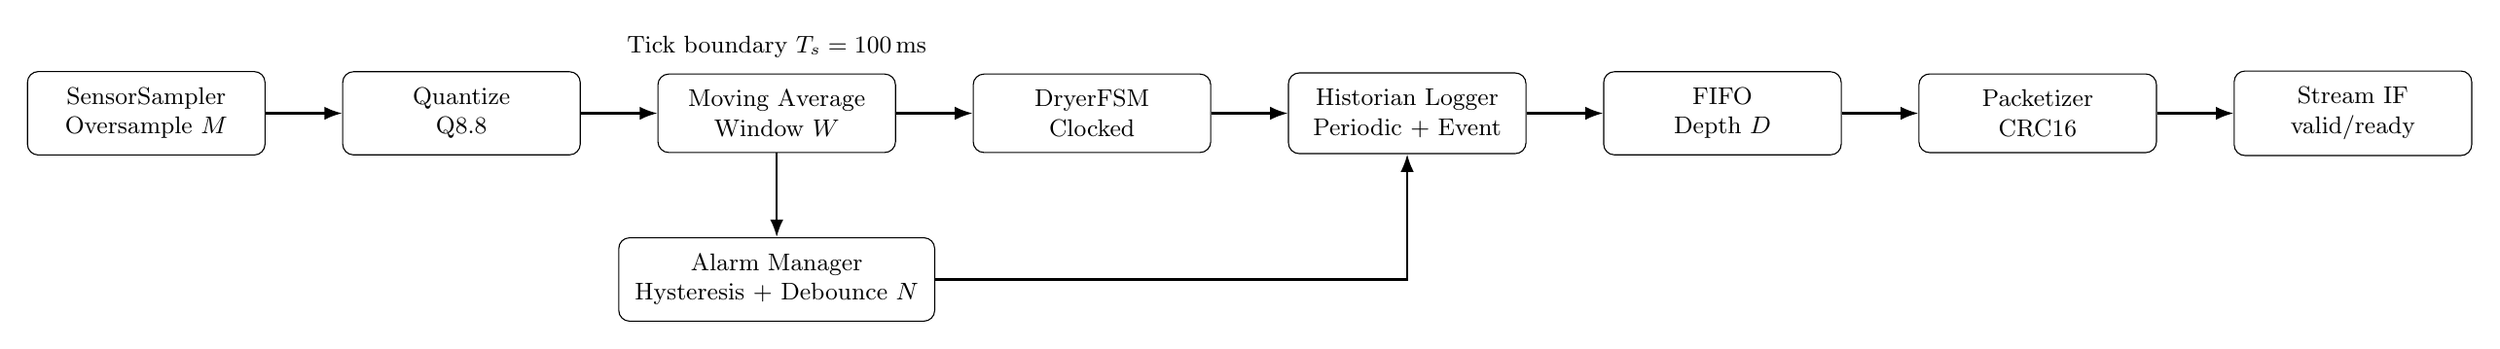
\begin{tikzpicture}[
  font=\small,
  box/.style={draw, rounded corners, align=center, minimum height=0.9cm, minimum width=3.1cm, inner sep=6pt},
  arr/.style={-Latex, thick}
]
\node[box] (sampler) {SensorSampler\\Oversample $M$};
\node[box, right=1.0cm of sampler] (q) {Quantize\\Q8.8};
\node[box, right=1.0cm of q] (ma) {Moving Average\\Window $W$};
\node[box, right=1.0cm of ma] (fsm) {DryerFSM\\Clocked};
\node[box, right=1.0cm of fsm] (logger) {Historian Logger\\Periodic + Event};
\node[box, right=1.0cm of logger] (fifo) {FIFO\\Depth $D$};
\node[box, right=1.0cm of fifo] (pkt) {Packetizer\\CRC16};
\node[box, right=1.0cm of pkt] (stream) {Stream IF\\valid/ready};

\node[box, below=1.1cm of ma] (alarm) {Alarm Manager\\Hysteresis + Debounce $N$};

\draw[arr] (sampler) -- (q);
\draw[arr] (q) -- (ma);
\draw[arr] (ma) -- (fsm);
\draw[arr] (fsm) -- (logger);
\draw[arr] (logger) -- (fifo);
\draw[arr] (fifo) -- (pkt);
\draw[arr] (pkt) -- (stream);

\draw[arr] (ma) -- (alarm);
\draw[arr] (alarm.east) -| (logger.south);

\node[align=center] at (ma.north) [yshift=10pt] {Tick boundary $T_s = 100\,\mathrm{ms}$};
\end{tikzpicture}%
}
\caption{Top level architecture with tick driven datapath and event coupling.}
\label{fig:block_diagram}
\end{figure}

\subsection{Record and Frame Interfaces}
The internal payload is a fixed width record. Externally the packetizer streams bytes. In RTL terms:
\begin{itemize}
    \item FIFO write port: \texttt{wr\_en}, \texttt{wr\_data[255:0]}, explicit drop on full.
    \item FIFO read port: \texttt{rd\_valid} when occupancy non zero, \texttt{rd\_data}, \texttt{rd\_pop} asserted when frame transmission completes.
    \item Stream port: \texttt{valid}, \texttt{ready}, \texttt{data[7:0]}.
\end{itemize}

\subsection{Simulation Generated Record Layout}
\begin{figure}[H]
    \centering
    \caption{Historian record layout (fixed width payload).}
    \footnotesize
    \verbatiminput{\builddir/tables/record_layout.txt}
    \label{fig:record_layout}
\end{figure}

% ==============================================================================
\section{Methodology and RTL Style Modeling Approach}
% ==============================================================================

\subsection{Deterministic Scheduling and Tick Semantics}
Primary tick period: $T_s = 100\,\mathrm{ms}$. This is treated as a synchronous cycle boundary for all sequential state. Within one tick, the model executes a fixed ordering of operations:
\begin{enumerate}
    \item Sensor sampling with optional oversampling (subsamples) and averaging.
    \item Fixed point conversion to Q8.8 integers.
    \item Per channel moving average filtering implemented as an integer accumulator and circular buffer.
    \item Control FSM step producing actuator outputs.
    \item Alarm manager step evaluating latched alarms using debounce counters and set clear thresholds.
    \item Historian record generation: one periodic record per tick and an additional record on any alarm rising edge.
    \item FIFO push of generated records; explicit drop on overflow.
    \item Packetizer step: if idle and FIFO non empty and ready asserted, construct a frame for FIFO head; if active and ready asserted, transmit up to a per tick byte budget; when complete, pop FIFO and account for latency.
\end{enumerate}

This schedule resembles a synthesizable multi stage pipeline with explicit combinational and sequential boundaries.

\subsection{Fixed Width Arithmetic and Saturations}
Sensor values are represented in Q8.8 fixed point: a signed integer encodes a real value $x$ as
\[
x_q = \mathrm{round}(x \cdot 2^8),
\qquad
\hat{x} = x_q \cdot 2^{-8}.
\]
Quantization error is bounded by $|e_q| \le 2^{-9}$ in real units. For i16 record storage, values are saturated to $[-32768, 32767]$ prior to packing.

\subsection{Synthesizable Memory Structures}
The historian FIFO is a finite depth circular buffer with explicit read and write pointers and an occupancy counter. Push drops on full and increments a drop counter. Peek is used to start packetization without committing a pop until the full frame is transmitted. This models a design in which payload memory and the streaming datapath are decoupled but record lifetime is controlled by FIFO semantics.

% ==============================================================================
\section{Sampling Theory and Timestamp Resolution}
% ==============================================================================

\subsection{Sampling Period and Effective Rate}
Primary tick: $T_s = 100\,\mathrm{ms}$, therefore $f_s = 10\,\mathrm{Hz}$. Oversampling uses $M$ subsamples per tick:
\[
\bar{x}[k] = \frac{1}{M}\sum_{m=0}^{M-1} x\!\left(kT_s + m\frac{T_s}{M}\right),
\]
followed by quantization to Q8.8.

\subsection{Timestamp Model and Bounded Jitter}
Each record stores \texttt{ts\_ms} in milliseconds. The model sets:
\[
\texttt{ts\_ms}[k] = k \cdot T_s.
\]
A bounded jitter model for a physical gateway can be written as
\[
t_k = kT_s + \epsilon_k,
\quad
|\epsilon_k| \le \epsilon_{\max},
\]
with $\epsilon_k = 0$ in the simulation by construction.

% ==============================================================================
\section{Fixed Point Filtering and Quantization Error}
% ==============================================================================

\subsection{Moving Average Filter}
Moving average window length $W$. Synthesizable implementation uses circular buffer, accumulator $S[k]$, and the recurrence:
\[
S[k] = S[k-1] + x[k] - x[k-W],
\qquad
y[k] = \left\lfloor \frac{S[k]}{W} \right\rfloor.
\]

\subsection{Impulse Response and Group Delay}
The moving average has an effective group delay of approximately $(W-1)/2$ ticks:
\[
\tau_g \approx \frac{W-1}{2}\,T_s.
\]
For example, $W=8$ yields $\tau_g \approx 3.5 \cdot 0.1\,\mathrm{s} = 0.35\,\mathrm{s}$.

\subsection{Quantization Noise Bounds}
For Q8.8, the quantization error satisfies $|e_q| \le 2^{-9}$. The moving average output additionally incurs truncation from integer division.

% \subsection{Synthesizable Datapath View of the Moving Average}
% The moving average can be implemented with a subtract add accumulator and a circular buffer indexed by \texttt{idx}. The division by $W$ is modeled as an integer division. For power of two $W$, hardware can replace divide with a shift; otherwise it is a small divider or reciprocal multiply depending on constraints. In this simulation, $W$ is a configurable integer and division is exact integer division.

% \begin{figure}[H]
% \centering
% \begin{tikzpicture}[
%   node distance=1.1cm,
%   blk/.style={draw, rounded corners, minimum width=2.7cm, minimum height=0.9cm, align=center},
%   sm/.style={draw, rounded corners, minimum width=1.7cm, minimum height=0.8cm, align=center},
%   arr/.style={-Latex, thick}
% ]
% \node[blk] (x) {$x[k]$\\Q8.8};
% \node[sm, right=1.0cm of x] (sub) {$-$};
% \node[sm, above=0.9cm of sub] (old) {$x[k-W]$\\from buf};
% \node[sm, right=1.0cm of sub] (add) {$+$};
% \node[blk, right=1.0cm of add] (acc) {Accumulator\\$S[k]$};
% \node[blk, right=1.0cm of acc] (div) {Divide by $W$\\floor};
% \node[blk, right=1.0cm of div] (y) {$y[k]$\\Q8.8};

% \draw[arr] (x) -- (sub);
% \draw[arr] (old) -- (sub);
% \draw[arr] (sub) -- (add);
% \draw[arr] (acc) -- (add);
% \draw[arr] (add) -- (acc);
% \draw[arr] (acc) -- (div);
% \draw[arr] (div) -- (y);

% \node[blk, below=1.0cm of sub] (buf) {Circular Buffer\\len $W$};
% \draw[arr] (x) |- (buf.west);
% \draw[arr] (buf.north) -- (old);

% \node[align=center, below=0.35cm of buf] {\small Registers: \texttt{idx}, \texttt{S}, buf[$W$]};
% \end{tikzpicture}
% \caption{Moving average datapath in RTL terms (accumulate by subtracting the oldest sample and adding the newest).}
% \label{fig:ma_datapath}
% \end{figure}

\subsection{Synthesizable Datapath View of the Moving Average}

The moving average filter is implemented using a subtract add accumulator and a circular buffer indexed by \texttt{idx}. At each tick, the newest quantized sample $x[k]$ is added to the accumulator, while the oldest sample $x[k-W]$ stored in the buffer is subtracted. This structure avoids recomputing the full window sum and yields constant time per update.

The division by $W$ is modeled as an integer division with floor semantics. When $W$ is a power of two, this operation may be realized as a right shift in hardware; otherwise, it corresponds to a small divider or reciprocal multiply depending on design constraints. In this simulation, $W$ is a configurable integer and division is exact integer division.

All state elements are explicit and bounded: the accumulator register $S[k]$, the circular buffer of length $W$, and the buffer index \texttt{idx}. The datapath is fully synthesizable and maps directly to a single clocked RTL process.

\begin{figure}[H]
\centering
\resizebox{0.92\linewidth}{!}{%
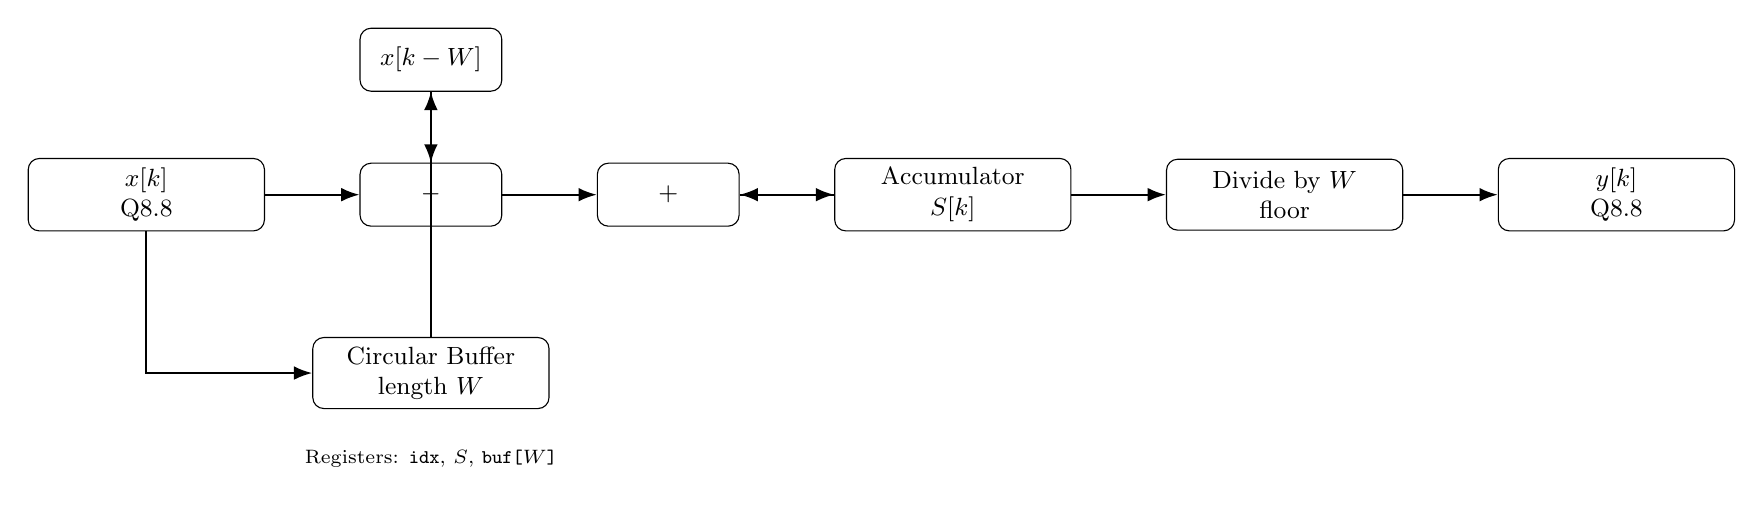
\begin{tikzpicture}[
  font=\small,
  blk/.style={draw, rounded corners, minimum width=3.0cm, minimum height=0.9cm, align=center},
  sm/.style={draw, rounded corners, minimum width=1.8cm, minimum height=0.8cm, align=center},
  arr/.style={-Latex, thick},
  lab/.style={font=\scriptsize, align=center}
]

% Main datapath
\node[blk] (xin) {$x[k]$\\Q8.8};
\node[sm, right=1.2cm of xin] (sub) {$-$};
\node[sm, right=1.2cm of sub] (add) {$+$};
\node[blk, right=1.2cm of add] (acc) {Accumulator\\$S[k]$};
\node[blk, right=1.2cm of acc] (div) {Divide by $W$\\floor};
\node[blk, right=1.2cm of div] (yout) {$y[k]$\\Q8.8};

% Circular buffer
\node[blk, below=1.4cm of sub] (buf) {Circular Buffer\\length $W$};
\node[sm, above=0.9cm of sub] (old) {$x[k-W]$};

% Connections
\draw[arr] (xin) -- (sub);
\draw[arr] (old) -- (sub);
\draw[arr] (sub) -- (add);
\draw[arr] (acc) -- (add);
\draw[arr] (add) -- (acc);
\draw[arr] (acc) -- (div);
\draw[arr] (div) -- (yout);

\draw[arr] (xin) |- (buf.west);
\draw[arr] (buf.north) -- (old);

% State annotation
\node[lab, below=0.4cm of buf] {Registers: \texttt{idx}, $S$, \texttt{buf[$W$]}};

\end{tikzpicture}%
}
\caption{Synthesizable moving average datapath using subtract add accumulation and a circular buffer.}
\label{fig:ma_datapath}
\end{figure}


\begin{figure}[htbp]
    \centering
    \includegraphics[width=0.86\linewidth]{sensor_temp_raw_vs_filt.png}
    \caption{Temperature raw vs filtered output (Q8.8 interpreted as Celsius).}
    \label{fig:temp_filt}
\end{figure}

\begin{figure}[htbp]
    \centering
    \includegraphics[width=0.86\linewidth]{sensor_moist_raw_vs_filt.png}
    \caption{Moisture raw vs filtered output (Q8.8 interpreted as percent).}
    \label{fig:moist_filt}
\end{figure}

\begin{figure}[htbp]
    \centering
    \includegraphics[width=0.86\linewidth]{sensor_press_raw_vs_filt.png}
    \caption{Pressure raw vs filtered output (Q8.8 interpreted as kPa).}
    \label{fig:press_filt}
\end{figure}

\begin{figure}[htbp]
    \centering
    \includegraphics[width=0.86\linewidth]{sensor_vib_raw_vs_filt.png}
    \caption{Vibration raw vs filtered output (Q8.8 interpreted as arbitrary units).}
    \label{fig:vib_filt}
\end{figure}

% ==============================================================================
\section{FSM Design and Timing Behavior}
% ==============================================================================

\subsection{State Encoding and Transitions}
Control logic is a clocked FSM with five states: IDLE, RAMP, STEADY, FAULT, COOLDOWN. Transitions are driven by filtered sensor values and dwell counters.

\subsection{Actuator Outputs and Safety}
Actuator outputs are Mealy style, depending on state and internal counters. Fault transitions have highest precedence; if a fault condition is detected, the state transitions to FAULT immediately.

\subsection{State Diagram (Control FSM)}
\begin{figure}[H]
\centering
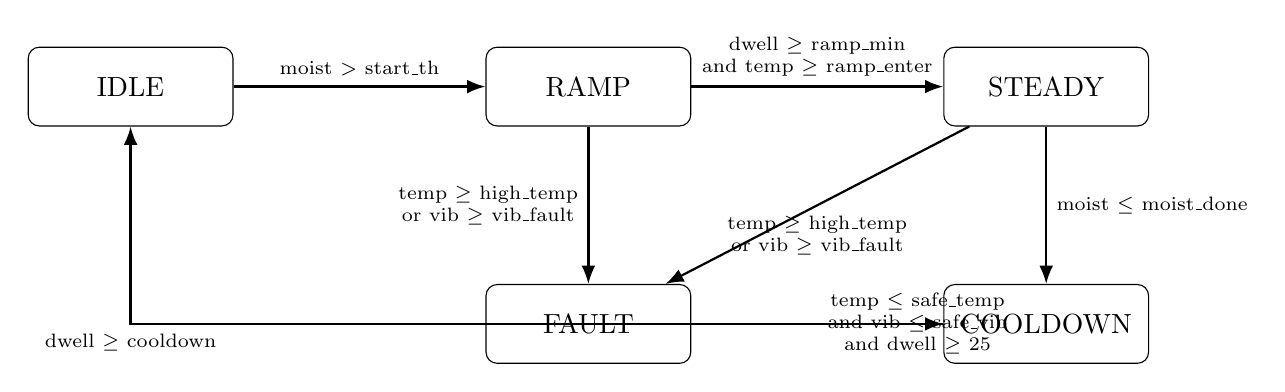
\begin{tikzpicture}[
  st/.style={draw, rounded corners, minimum width=2.6cm, minimum height=1.0cm, align=center},
  arr/.style={-Latex, thick},
  lab/.style={font=\scriptsize, align=center}
]
\node[st] (idle) {IDLE};
\node[st, right=3.2cm of idle] (ramp) {RAMP};
\node[st, right=3.2cm of ramp] (steady) {STEADY};
\node[st, below=2.0cm of steady] (cool) {COOLDOWN};
\node[st, below=2.0cm of ramp] (fault) {FAULT};

\draw[arr] (idle) -- node[lab, above] {moist $>$ start\_th} (ramp);
\draw[arr] (ramp) -- node[lab, above] {dwell $\ge$ ramp\_min\\and temp $\ge$ ramp\_enter} (steady);
\draw[arr] (steady) -- node[lab, right] {moist $\le$ moist\_done} (cool);
\draw[arr] (cool) -| node[lab, below] {dwell $\ge$ cooldown} (idle);

\draw[arr] (ramp) -- node[lab, left] {temp $\ge$ high\_temp\\or vib $\ge$ vib\_fault} (fault);
\draw[arr] (steady) -- node[lab, below] {temp $\ge$ high\_temp\\or vib $\ge$ vib\_fault} (fault);
\draw[arr] (fault) -- node[lab, right] {temp $\le$ safe\_temp\\and vib $\le$ safe\_vib\\and dwell $\ge$ 25} (cool);
\end{tikzpicture}
\caption{Dryer control FSM state diagram (conditions match the simulation logic).}
\label{fig:fsm_diagram}
\end{figure}

\subsection{FSM as a Synchronous Next-State Function}
A synthesizable FSM is typically expressed as:
\[
s[k+1] = \delta\left(s[k],\,x[k]\right),
\qquad
u[k] = \lambda\left(s[k],\,x[k]\right),
\]
where $s$ is the discrete state register, $x$ are filtered sensor inputs, and $u$ are actuator outputs. The dwell counter is an additional state register updated per tick:
\[
d[k+1] =
\begin{cases}
0, & \text{if state transition occurs} \\
d[k] + 1, & \text{otherwise}
\end{cases}
\]

\subsection{Actuator Output Logic (Interpretation)}
The simulation logic yields actuator behaviors that can be described as:
\begin{itemize}
    \item IDLE: low fan, heater off, valve closed.
    \item RAMP: heater on, fan medium, valve closed.
    \item STEADY: fan high; heater is duty-modulated in-band; valve depends on moisture threshold.
    \item FAULT: heater off; fan max; valve open.
    \item COOLDOWN: heater off; fan high; valve open; return to IDLE after cooldown dwell.
\end{itemize}

\begin{figure}[htbp]
    \centering
    \includegraphics[width=\linewidth]{fsm_timeline.png}
    \caption{FSM state timeline at tick resolution.}
    \label{fig:fsm_timeline}
\end{figure}

\begin{figure}[htbp]
    \centering
    \includegraphics[width=\linewidth]{actuators.png}
    \caption{Actuator outputs driven by the control FSM.}
    \label{fig:actuators}
\end{figure}

% ==============================================================================
\section{Alarm Debounce Derivation}
% ==============================================================================

\subsection{Hysteresis and Debounce}
Each alarm is a latched comparator with separate set and clear thresholds. If unlatched and the set condition holds for $N$ consecutive ticks, the latch becomes 1. If latched and the clear condition holds for $N$ consecutive ticks, the latch becomes 0. With $T_s = 100\,\mathrm{ms}$ and $N=3$, the minimum persistent excursion required is $N T_s = 300\,\mathrm{ms}$.

\subsection{Debounce as a Small Two-State FSM}
The debouncer can be viewed as a two-state FSM per alarm bit with an $N$-tick counter. A compact model is:
\[
\texttt{cnt}[k+1] =
\begin{cases}
\texttt{cnt}[k] + 1, & \text{if condition holds} \\
0, & \text{otherwise}
\end{cases}
\]
and the latch toggles when $\texttt{cnt} \ge N$ under the appropriate set or clear condition.

\begin{figure}[H]
\centering
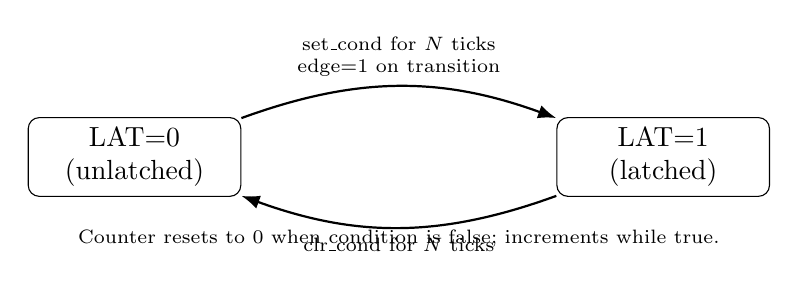
\begin{tikzpicture}[
  st/.style={draw, rounded corners, minimum width=2.7cm, minimum height=1.0cm, align=center},
  arr/.style={-Latex, thick},
  lab/.style={font=\scriptsize, align=center}
]
\node[st] (low) {LAT=0\\(unlatched)};
\node[st, right=4.0cm of low] (high) {LAT=1\\(latched)};

\draw[arr] (low) to[bend left=20] node[lab, above] {set\_cond for $N$ ticks\\edge=1 on transition} (high);
\draw[arr] (high) to[bend left=20] node[lab, below] {clr\_cond for $N$ ticks} (low);

\node[lab, below=0.8cm of $(low)!0.5!(high)$] {Counter resets to 0 when condition is false; increments while true.};
\end{tikzpicture}
\caption{Debounced hysteresis latch interpreted as a two-state FSM with an $N$-tick counter.}
\label{fig:debounce_fsm}
\end{figure}

\subsection{Event Detection}
An alarm event is defined as a rising edge (latch transition 0 to 1). A priority encoder assigns a single event code per tick in the presence of multiple edges.

\begin{figure}[htbp]
    \centering
    \includegraphics[width=\linewidth]{alarms_masks.png}
    \caption{Alarm latch outputs and rising edge detections.}
    \label{fig:alarms}
\end{figure}

% ==============================================================================
\section{Historian Logger and FIFO Sizing}
% ==============================================================================

\subsection{Record Generation Rate}
Attempted record rate is $R_{\text{in}} = R_p + R_e$, where $R_p = 1/T_s = 10\,\mathrm{Hz}$ is the periodic rate and $R_e$ is the event driven increment. Let $A[k]$ be the number of records attempted at tick $k$ (1 or 2), and let $D[k]$ be the number of records dequeued for transmission completion at tick $k$ (0 or 1). The occupancy recurrence is:
\[
O[k+1] = \min(D_{\text{FIFO}},\, O[k] + A[k] - D[k]),
\]
with explicit drops on overflow when $O[k] = D_{\text{FIFO}}$ and $A[k] > D[k]$.

\subsection{FIFO Circuit Sketch (Synthesizable View)}
\begin{figure}[H]
\centering
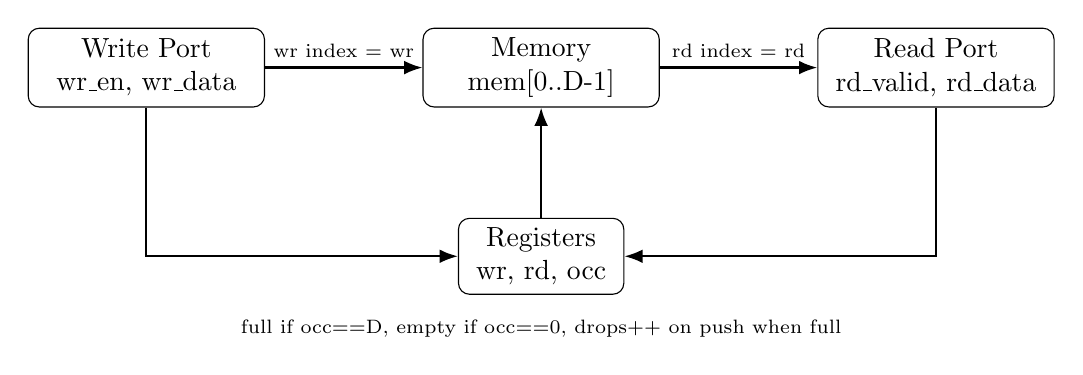
\begin{tikzpicture}[
  blk/.style={draw, rounded corners, minimum width=3.0cm, minimum height=1.0cm, align=center},
  sm/.style={draw, rounded corners, minimum width=2.1cm, minimum height=0.9cm, align=center},
  arr/.style={-Latex, thick},
  lab/.style={font=\scriptsize}
]
\node[blk] (wr) {Write Port\\wr\_en, wr\_data};
\node[blk, right=2.0cm of wr] (mem) {Memory\\mem[0..D-1]};
\node[blk, right=2.0cm of mem] (rd) {Read Port\\rd\_valid, rd\_data};

\node[sm, below=1.4cm of mem] (ptr) {Registers\\wr, rd, occ};

\draw[arr] (wr) -- node[lab, above] {wr index = wr} (mem);
\draw[arr] (mem) -- node[lab, above] {rd index = rd} (rd);

\draw[arr] (ptr) -- (mem);
\draw[arr] (wr) |- (ptr.west);
\draw[arr] (rd) |- (ptr.east);

\node[lab, below=0.2cm of ptr] {full if occ==D, empty if occ==0, drops++ on push when full};
\end{tikzpicture}
\caption{Historian FIFO modeled as circular memory with pointers and occupancy register.}
\label{fig:fifo_circuit}
\end{figure}

\begin{figure}[htbp]
    \centering
    \includegraphics[width=\linewidth]{fifo_occupancy_and_drops.png}
    \caption{FIFO occupancy and record drops over time.}
    \label{fig:fifo}
\end{figure}

% ==============================================================================
\section{Packetizer and CRC Polynomial}
% ==============================================================================

\subsection{Frame Format and CRC16}
Frame format:
\[
\texttt{[SYNC][HEADER][PAYLOAD][CRC16]}.
\]
SYNC bytes are \texttt{0xA5 0x5A}. CRC16 CCITT polynomial over GF(2):
\[
G(x) = x^{16} + x^{12} + x^5 + 1.
\]
CRC is computed over \texttt{HEADER || PAYLOAD} (SYNC excluded), using the parameters embedded in the configuration.

\subsection{CRC Bitwise Update as an LFSR (Circuit Perspective)}
A common RTL implementation uses a 16-bit shift register with conditional XOR taps according to $G(x)$. In the non-reflected CCITT form used here, each input bit is processed MSB-first with a feedback bit. The simulation uses the exact same bitwise behavior.

\begin{figure}[H]
\centering
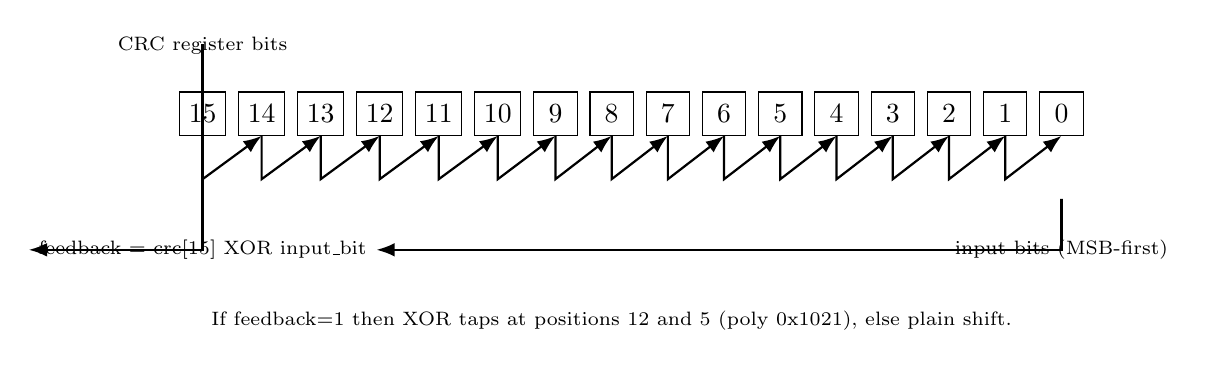
\begin{tikzpicture}[
  bit/.style={draw, minimum width=0.55cm, minimum height=0.55cm, align=center},
  arr/.style={-Latex, thick},
  lab/.style={font=\scriptsize}
]
\node[bit] (b15) {15};
\node[bit, right=0.15cm of b15] (b14) {14};
\node[bit, right=0.15cm of b14] (b13) {13};
\node[bit, right=0.15cm of b13] (b12) {12};
\node[bit, right=0.15cm of b12] (b11) {11};
\node[bit, right=0.15cm of b11] (b10) {10};
\node[bit, right=0.15cm of b10] (b9) {9};
\node[bit, right=0.15cm of b9] (b8) {8};
\node[bit, right=0.15cm of b8] (b7) {7};
\node[bit, right=0.15cm of b7] (b6) {6};
\node[bit, right=0.15cm of b6] (b5) {5};
\node[bit, right=0.15cm of b5] (b4) {4};
\node[bit, right=0.15cm of b4] (b3) {3};
\node[bit, right=0.15cm of b3] (b2) {2};
\node[bit, right=0.15cm of b2] (b1) {1};
\node[bit, right=0.15cm of b1] (b0) {0};

\node[lab, above=0.35cm of b15] {CRC register bits};

% Shift arrows
\foreach \a/\b in {b15/b14,b14/b13,b13/b12,b12/b11,b11/b10,b10/b9,b9/b8,b8/b7,b7/b6,b6/b5,b5/b4,b4/b3,b3/b2,b2/b1,b1/b0} {
  \draw[arr] (\a.south) -- ++(0,-0.55) -- ++(0.0,0) -- (\b.south);
}

% Feedback concept
\node[lab, below=1.2cm of b15] (fb) {feedback = crc[15] XOR input\_bit};
\draw[arr] (b15.north) -- ++(0,0.6) |- (fb.west);

\node[lab, below=1.2cm of b0] (in) {input bits (MSB-first)};
\draw[arr] (in.north) -- ++(0,0.4) |- (fb.east);

\node[lab, below=2.1cm of b8] {If feedback=1 then XOR taps at positions 12 and 5 (poly 0x1021), else plain shift.};
\end{tikzpicture}
\caption{CRC16-CCITT modeled as an LFSR-like shift register with conditional XOR taps (conceptual circuit sketch).}
\label{fig:crc_lfsr}
\end{figure}

\subsection{Embedded CRC Configuration and Validation Vectors}
\begin{figure}[H]
    \centering
    \caption{CRC configuration (embedded JSON).}
    \footnotesize
    \verbatiminput{\builddir/tables/crc_config.json}
\end{figure}

\begin{figure}[H]
    \centering
    \caption{CRC validation vectors (embedded CSV excerpt).}
    \footnotesize
    \verbatiminput{\builddir/tables/crc_vectors.csv}
\end{figure}

% ==============================================================================
\section{Protocol Multiplexer}
% ==============================================================================

Two protocol header formats differ structurally but share payload and CRC mechanism:
\begin{itemize}
    \item \textbf{Modbus-like:} \texttt{[addr][func][len\_lo][len\_hi]} (4 bytes)
    \item \textbf{CIP-like:} \texttt{[service][class][instance][len\_lo][len\_hi]} (5 bytes)
\end{itemize}

\begin{figure}[htbp]
    \centering
    \includegraphics[width=\linewidth]{protocol_selection_over_time.png}
    \caption{Protocol multiplexer selection over time.}
    \label{fig:protocols}
\end{figure}

% ==============================================================================
\section{Streaming Handshake, Throughput, and Latency Bounds}
% ==============================================================================

\subsection{Handshake Model}
The valid and ready handshake models streaming output under backpressure. A frame starts only when the packetizer is idle, FIFO is non empty, and ready is high. When active, the packetizer transmits up to a per tick byte budget while ready remains asserted.

\subsection{Packetizer Micro-FSM (Idle vs Sending)}
The packetizer is naturally modeled as a two-state FSM:
\begin{itemize}
    \item IDLE: if FIFO non-empty and ready=1, capture header and payload, compute CRC, start sending, assert start\_fire.
    \item SENDING: each tick, if ready=1, transmit up to $B$ bytes; when frame bytes complete, pop FIFO and return to IDLE.
\end{itemize}

\begin{figure}[H]
\centering
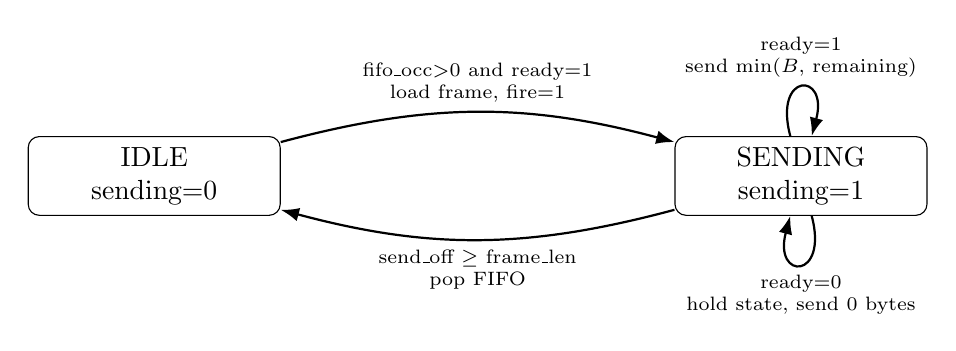
\begin{tikzpicture}[
  st/.style={draw, rounded corners, minimum width=3.2cm, minimum height=1.0cm, align=center},
  arr/.style={-Latex, thick},
  lab/.style={font=\scriptsize, align=center}
]
\node[st] (idle) {IDLE\\sending=0};
\node[st, right=5.0cm of idle] (send) {SENDING\\sending=1};

\draw[arr] (idle) to[bend left=15] node[lab, above] {fifo\_occ$>$0 and ready=1\\load frame, fire=1} (send);
\draw[arr] (send) to[bend left=15] node[lab, below] {send\_off $\ge$ frame\_len\\pop FIFO} (idle);

\draw[arr] (send) to[loop above] node[lab, above] {ready=1\\send min($B$, remaining)} (send);
\draw[arr] (send) to[loop below] node[lab, below] {ready=0\\hold state, send 0 bytes} (send);
\end{tikzpicture}
\caption{Packetizer micro-FSM controlling start, byte transmission, and FIFO pop.}
\label{fig:pkt_fsm}
\end{figure}

\begin{figure}[htbp]
    \centering
    \includegraphics[width=\linewidth]{handshake_valid_ready_fire.png}
    \caption{Valid and ready handshake behavior.}
    \label{fig:handshake}
\end{figure}

\subsection{Backpressure Adjusted Service Bound}
Let $\rho$ denote the fraction of ticks where ready is high. Let $B$ be the byte budget per tick and let $L_f$ be the frame length in bytes. A lower bound on the number of ticks required per frame is $\lceil L_f / B \rceil$, so a crude service rate bound is
\[
R_{\text{svc}} \lesssim \frac{\rho}{\lceil L_f/B \rceil}\cdot \frac{1}{T_s}.
\]
When $R_{\text{in}} > R_{\text{svc}}$ in expectation, FIFO occupancy grows toward capacity, leading to drops.

\subsection{Latency Definition and Measurement}
Latency is measured in ticks from record enqueue to record dequeue (pop) when the frame completes transmission. If a record is enqueued at tick $k_e$ and popped at tick $k_p$, then:
\[
L = k_p - k_e.
\]
Separate latency series are tracked for periodic records and event records.

\begin{figure}[htbp]
    \centering
    \includegraphics[width=\linewidth]{throughput_bytes.png}
    \caption{Bytes transmitted per tick under backpressure.}
    \label{fig:throughput}
\end{figure}

\begin{figure}[htbp]
    \centering
    \includegraphics[width=\linewidth]{latency_periodic_hist.png}
    \caption{Latency histogram for periodic records (ticks).}
    \label{fig:lat_hist_p}
\end{figure}

% NOTE: Event histogram is intentionally omitted when it has no samples.
% \begin{figure}[htbp]
%     \centering
%     \includegraphics[width=\linewidth]{latency_event_hist.png}
%     \caption{Latency histogram for event records (ticks).}
%     \label{fig:lat_hist_e}
% \end{figure}

% ==============================================================================
\section{Verification Strategy and Determinism}
% ==============================================================================

The simulation uses a fixed random seed to produce deterministic noise processes. With identical seed and configuration, outputs are reproducible.

\subsection{Pseudo RTL Listings}

\begin{lstlisting}[caption=Synthesizable Moving Average Update (Q8.8)]
/* State: int32 acc; int16 buf[W]; int idx; */
old = buf[idx];
acc = acc - old + x_q88;
buf[idx] = x_q88;
idx = (idx + 1) % W;
y_q88 = (int16)(acc / W); /* integer division */
\end{lstlisting}

\begin{lstlisting}[caption=Debounced Latch with Hysteresis]
/* State: bit latched; uint cnt; */
edge = 0;
if (!latched) {
  if (set_cond(x_q88)) {
    cnt++;
    if (cnt >= N) { latched = 1; cnt = 0; edge = 1; }
  } else cnt = 0;
} else {
  if (clr_cond(x_q88)) {
    cnt++;
    if (cnt >= N) { latched = 0; cnt = 0; }
  } else cnt = 0;
}
\end{lstlisting}

\begin{lstlisting}[caption=CRC16 CCITT Bitwise Update]
crc = 0xFFFF;
for each byte b in (header || payload) {
  crc ^= ((uint16)b << 8);
  repeat 8 times {
    if (crc & 0x8000) crc = (crc << 1) ^ 0x1021;
    else              crc = (crc << 1);
    crc &= 0xFFFF;
  }
}
\end{lstlisting}

\begin{lstlisting}[caption=FIFO Push Pop Semantics]
/* State: mem[D], rd, wr, occ, drops */
push(item):
  if (occ == D) { drops++; return 0; }
  mem[wr] = item; wr = (wr + 1) % D; occ++; return 1;

peek():
  if (occ == 0) return (0, null);
  return (1, mem[rd]);

pop():
  if (occ == 0) return (0, null);
  item = mem[rd]; rd = (rd + 1) % D; occ--; return (1, item);
\end{lstlisting}

% ==============================================================================
\section{Results and Discussion}
% ==============================================================================

\subsection{Sensor Dynamics}
The sensor generator includes deterministic disturbance windows that create excursions in temperature, vibration, and moisture, permitting observation of filtering, control response, and alarm behavior.

\begin{figure}[htbp]
    \centering
    \includegraphics[width=\linewidth]{zoom_temp_drift_fault.png}
    \caption{Zoom: Temperature drift and vibration disturbance.}
    \label{fig:zoom1}
\end{figure}

\begin{figure}[htbp]
    \centering
    \includegraphics[width=\linewidth]{zoom_moisture_drop.png}
    \caption{Zoom: Moisture transient and control response.}
    \label{fig:zoom2}
\end{figure}

\begin{figure}[htbp]
    \centering
    \includegraphics[width=\linewidth]{zoom_disturbance_1.png}
    \caption{Zoom: Vibration disturbance segment and system response.}
    \label{fig:zoom3}
\end{figure}

\subsection{Run Summary (Embedded)}
\begin{figure}[H]
    \centering
    \caption{Run summary (embedded JSON).}
    \footnotesize
    \verbatiminput{\builddir/tables/run_summary.json}
\end{figure}

\subsection{Configuration Metadata (Embedded)}
\begin{figure}[H]
    \centering
    \caption{Configuration metadata (embedded CSV).}
    \footnotesize
    \verbatiminput{\builddir/tables/config_metadata.csv}
\end{figure}

\subsection{Thresholds (Embedded)}
\begin{figure}[H]
    \centering
    \caption{Alarm thresholds (embedded CSV).}
    \footnotesize
    \verbatiminput{\builddir/tables/thresholds.csv}
\end{figure}

% ==============================================================================
\section{Conclusion}
% ==============================================================================
EDISGA demonstrates a complete event driven sensor gateway datapath consistent with synthesizable logic: tick based sampling, fixed point filtering, a clocked control FSM, debounced alarm latching with edge capture, deterministic record logging into a bounded FIFO with explicit overflow, and packetization with CRC into a valid and ready streaming interface under throughput constraints. The embedded figures and tables provide trace level evidence for control behavior, alarm dynamics, buffering effects under backpressure, and integrity checks via CRC configuration and validation vectors.

\end{document}
